\documentclass[11pt]{article}

\usepackage{october}
\usepackage{lineno}
% For BJPS
% \hyphenpenalty=10000
% \hbadness=10000

\begin{document}
\setpagewiselinenumbers
\modulolinenumbers[5]
\linenumbers
% For BJPS
% \raggedright
% \doublespacing

% y=3;z=4;pdftk A=epsa-jeffrey-conditioning\ \($y\).pdf cat A1-$z output wc-out.pdf

\title{Monotone Invariance}
\author{Stefan Lukits}
\date{}
\maketitle
% \newcounter{expls}
% \doublespacing

% \begin{abstract}
%   {\noindent}
% \end{abstract}

Now turning to the woes of the information theorist. Given the
asymmetric similarity measure of probability distributions that
information theory requires (the Kullback-Leibler divergence), a prior
probability distribution $P$ may be closer to a posterior probability
distribution $Q$ than $Q$ is to $P$ if their roles (prior-posterior)
are reversed. That is just what we would expect. The problem is that
there is another posterior probability distribution $R$ where the
situation is just the opposite: prior $P$ is further away from
posterior $R$ than prior $R$ is from posterior $P$. And whether a
probability distribution different from $P$ is of the $Q$-type or of
the $R$-type escapes any epistemic intuition.

Let me put this differently to emphasize the gravity of the situation
for information theory. For simplicity, let us consider probability
distributions and their associated credence functions on an event
space with three atoms $\Omega=\{\omega_{1},\omega_{2},\omega_{3}\}$.
The simplex $\mathbb{S}^{2}$ represents all of these probability
distributions. Every point $p$ in $\mathbb{S}^{2}$ representing a
probability distribution $P$ induces a partition on $\mathbb{S}^{2}$
into points that are symmetric to $p$, positively skew-symmetric to
$p$, and negatively skew-symmetric to $p$ given the topology of
information theory.

In other words, if

\begin{equation}
  \label{eq:sksy}
  \Delta_{P}(P')=D_{\mbox{\tiny KL}}(P',P)-D_{\mbox{\tiny KL}}(P,P'),
\end{equation}

then, holding $P$ fixed, $\mathbb{S}^{2}$ is partitioned into three
regions, $\Delta^{-1}(\mathbb{R}_{>0})$,
$\Delta^{-1}(\mathbb{R}_{<0})$, and $\Delta^{-1}(\{0\})$. One could
have a simple epistemic intuition such as \qnull{it takes less to
  update from a more uncertain probability distribution to a more
  certain probability distribution than the reverse direction,} where
the degree of certainty in a probability distribution is measured by
its entropy. This simple intuition accords with what we said about
extreme probabilities and it holds true for the asymmetric distance
measure defined by the Kullback-Leibler divergence in the
two-dimensional case where $\Omega$ has only two elements (see
appendix \ref{app:asytwodims}).

In higher-dimensional cases, however, the tripartite partition induced
by (\ref{eq:sksy}) is non-trivial---some probability distributions are
of the $Q$-type, some are of the $R$-type, and it is difficult to
think of an epistemic distinction between them that does not already
presuppose information theory. See figure \ref{fig:concat} for
graphical illustration of this point.

On any account of well-behaved and ill-behaved asymmetries, the
Kullback-Leibler divergence is ill-behaved. Of the four axioms as
listed by Ralph Kopperman for a distance measure $d$ (see
\scite{8}{kopperman88}{89}), the Kullback-Leibler divergence violates
both symmetry and triangularity, making it a \qnull{semi-quasimetric}:

\begin{enumerate}[(m1)]
\item $d(x,x)=0$
\item $d(x,z)\leq{}d(x,y)+d(y,z)$ (triangularity)
\item $d(x,y)=d(y,x)$ (symmetry)
\item $d(x,y)=0$ implies $x=y$ (separation)
\end{enumerate}

Kopperman's subjective is primarily to rescue continuity, uniform
continuity, Cauchy sequences, and limits for topologies induced by
distance measures which violate triangularity, symmetry, and/or
separation. Kopperman does not touch the first axiom, while in the
psychological literature (see especially \scite{7}{tversky77}{})
self-similarity is an important topic. This is why an initially
promising approach to asymmetric modeling in Hilbert spaces by 
Chino (see \scite{7}{chino78}{}; \scite{7}{chino90}{};
\scite{7}{chinoshiraiwa93}{}; and \scite{7}{saburichino08}{}) will not
help us to distinguish well-behaved and ill-behaved asymmetries
between probability distributions. I will explain the reasons in a
brief excursus, which is illuminative of classification for
asymmetries and has implications for Chino's modeling proposal as a
whole. 

The failure of Chino's modeling approach to make useful distinctions
among asymmetric distance measures between probability distributions
leads us to the more complex theory of information geometry and
differentiable manifolds. Both the results of Shun-ichi Amari (see
\scite{7}{amari85}{}; and \scite{7}{amarinagaoka00}{}) and Nikolai
Chentsov (see \scite{7}{chentsov82}{}) serve to highlight the special
properties of the Kullback-Leibler divergence, not without elevating
the discussion to a level of mathematical sophistication, however,
where it is difficult to retain the appeal to epistemic intuitions.
Information geometry considers probability distributions as
differentiable manifolds equipped with a Riemannian metric. This
metric, however, is Fisher's information metric, not the
Kullback-Leibler divergence, and it is defined on the tangent space of
the simplex representing finite-dimensional probability distributions.
There is a sense in which the Fisher information metric is the
derivative of the Kullback-Leibler divergence, and so the connection
to epistemic intuitions can be re-established.

What is missing is the uniqueness results for the Kullback-Leibler
divergence to show that despite its ill behaviour the Kullback-Leibler
is the right asymmetric distance measure on which to base inference
and updating. Here I will help myself to Chentsov's theory of monotone
invariance, which will also give us another strong indicator against
the geometry of reason that the distance measure between probability
distributions needs to be asymmetrical. What Chentsov's theory does
for us more specifically, however, is to provide us with a reason to
reject the idea that there might be well-behaved asymmetry measures
which can do the job as well as the ill-behaved distance measures of
information theory. Three subsections are to follow. one on Chino's
asymmetric modeling approach, which will motivate the subsequent two
subsections on information geometry (primarily using Amari's results)
and monotone invariance (primarily using Chentsov's results).

\subsubsection{The Hermitian Form Model}
\label{subsubsec:hfm}

The Kullback-Leibler divergence not only violates symmetry, but also
triangularity and transitivity. As a \qnull{semi-quasimetric,} it is
about as ill-behaved as a distance measure can get. Triangularity and
transitivity are properties that we may reasonably expect from a
distance measure on probability distributions, even if we want
asymmetry. After all, a violation of triangularity means that updating
from $R_{1}$ to $R_{2}$ and then from $R_{2}$ to $R_{3}$ is somehow less of an effort
than updating from $R_{1}$ to $R_{3}$ directly. For example,

\begin{equation}
  \label{eq:triang}
  D_{\mbox{\tiny KL}}(R_{1},R_{3})>D_{\mbox{\tiny KL}}(R_{1},R_{2})+D_{\mbox{\tiny KL}}(R_{2},R_{3})
\end{equation}

for

\begin{equation}
  \label{eq:triangviol}
    R_{1}=\left(\frac{1}{3},\frac{1}{3},\frac{1}{3}\right) \hspace{.5in}
    R_{2}=\left(\frac{2}{5},\frac{2}{5},\frac{1}{5}\right)  \hspace{.5in}
    R_{3}=\left(\frac{4}{5},\frac{1}{10},\frac{1}{10}\right).
\end{equation}

A violation of transitivity means that even though $P_{1}$ may be
asymmetrical to $P_{2}$ in favour of $P_{2}$ (it is somehow less of an
effort to get from $P_{1}$ to $P_{2}$ than from $P_{2}$ to $P_{1}$)
and $P_{2}$ may be asymmetrical to $P_{3}$ in favour of $P_{3}$,
$P_{1}$ is asymmetrical to $P_{3}$ in favour of $P_{1}$. Using
$\Delta$ defined in (\ref{eq:sksy}), for example,
$\Delta_{P_{3}}(P_{1})>0$ while $\Delta_{P_{2}}(P_{1})<0$ and
$\Delta_{P_{3}}(P_{2})<0$ given

\begin{equation}
  \label{eq:transviol}
    P_{1}=\left(\frac{1}{3},\frac{1}{3},\frac{1}{3}\right) \hspace{.5in}
    P_{2}=\left(\frac{1}{2},\frac{1}{4},\frac{1}{4}\right)  \hspace{.5in}
    P_{3}=\left(\frac{2}{5},\frac{2}{5},\frac{1}{5}\right).
\end{equation}

How counterintuitive this is (epistemically and otherwise) is
demonstrated by the fact that in MDS (the multi-dimensional scaling of
distance relationships) almost all asymmetric distance relationships
under consideration are transitive and triangular in nature (see, for
example, journal citation (Coombs, 1964), international trade (Chino,
1978), car switch (Harshman, Green, Wind, and Lundy, 1982), telephone
calls (Harshman and Lundy, 1984), and interaction or input-output flow
in migration, economic activity, and social mobility (Blau and Duncan,
1967 ; Coxon, 1982); flight time between two citie
s\scite{8}{gentleman06}{191}; mutual intelligibility between Swedish
and Danish \scite{8}{vanommenetal13}{193} Tobler's wind model,
Kopperman's cyclist). Asymmetric MDS is a promising approach to
classify some of these asymmetries in terms of their behaviour. This
subsection demonstrates that Chino's asymmetric MDS, both spatial and
non-spatial, fails to give us results. I am choosing Chino's approach
because it is the most general and most promising of all the different
asymmetric MDS models (see, for example, \scite{7}{chinoshiraiwa93}{},
where Chino manages to subsume many of the other approaches into his
own). 

Multi-dimensional scaling (MDS) visualizes similarity of individuals
in datasets. Various techniques are used in information visualization,
in particular to display the information contained in a proximity
matrix. When the proximity matrix is asymmetrical, we speak of
asymmetric MDS. These techniques can be spatial (see for example
\scite{7}{chino78}{}), where the proximity relationships are
visualized in two-dimensional or higher-dimensional space; or
non-spatial (see for example \scite{7}{chinoshiraiwa93}{}), where the
proximity relationships are used to identify data sets with abstract
spaces (in Chino's case, finite-dimensional complex Hilbert spaces)
and metrics defined on them.

The spatial approach in two dimensions fails right away for
information theory because it cannot visualize transitivity
violations. The hope for other types of asymmetric MDS is that it
would be able to distinguish between well-behaved and ill-behaved
asymmetries and either exclude or identify better-behaved candidates
than the Kullback-Leibler divergence for measuring the distance
between probability distributions. I will use Chino's most
sophisticated non-spatial account to show that asymmetric MDS cannot
solve this problem. For other asymmetric MDS note that with the
Hermitian Form Model Chino seeks to integrate and generalize over all
the other accounts. 

Assume a finity proximity matrix. I will work with two examples here
to avoid the detailed and abstract account provided by Chino. The
first example is

\begin{equation}
  \label{eq:simpromat}
D=\left[
      \begin{array}{ccc}
        0 & 2 & 3 \\
        3 & 0 & 1 \\
        -1 & 2 & 0 
      \end{array}
\right]
\end{equation}

and allows for easy calculations. The second example corresponds to
(\ref{eq:transviol}), the example for transitivity violation where

\begin{equation}
  \label{eq:dklpromat}
\hat{D}=\left[
      \begin{array}{ccc}
0.0000 &  0.0566 &  0.0487 \\
0.0589 &  0.0000 &  0.0499 \\
0.0437 &  0.0541 &  0.0000
      \end{array}
\right],
\end{equation}

and the elements of the matrix $\hat{d}_{jk}=D_{\mbox{\tiny KL}}(P_{j},P_{k})$.
Note that the diagonal elements are all zero, as no updating is
necessary to keep the probability distribution constant.

Chino first defines a symmetric matrix $S$ and a skew-symmetric matrix
$T$ corresponding to the proximity matrix such that $D=S+T$.

\begin{equation}
  \label{eq:skewsym}
  S=\frac{1}{2}(D+D')\mbox{ and }T=\frac{1}{2}(D-D').
\end{equation}

Note that $D'$ is the transpose of $D$, $S$ is a symmetric matrix, and
$T$ is a skew-symmetric matrix with $t_{jk}=-t_{kj}$. Next we define
the Hermitian matrix

\begin{equation}
  \label{eq:herm}
  H=S+iT,
\end{equation}

where $i$ is the imaginary unit. $H$ is a Hermitian matrix with
$h_{jk}=\overline{h_{kj}}$. Hermitian matrices are the complex
generalization of real symmetric matrices. They have special
properties (see Busby\tbd{cite}) which guarantee that the existence of
a unitary matrix $U$ such that 

\begin{equation}
  \label{eq:unitary}
  H=U\Lambda{}U^{*},
\end{equation}

where $\Lambda=\mbox{diag}(\lambda_{1},\ldots,\lambda_{n})$ with $n$
the dimension of $D$ and $\lambda_{k}$ the $k$-th eigenvalue of $H$.
$U$ is the matrix of eigenvectors with the $k$-th column being the
$k$-th eigenvector. $U^{*}$ is the conjugate transpose of $U$. Given
example (\ref{eq:simpromat}), the numbers look as follows:

\begin{equation}
  \label{eq:simh}
H=\frac{1}{2}\left[
      \begin{array}{ccc}
        0 & 5-i & 2+4i \\
        5+i & 0 & 3-i \\
        2-4i & 3+i & 0 
      \end{array}
\right]
\end{equation}

and

\begin{equation}
  \label{eq:simu}
U=\left[
      \begin{array}{ccc}
   0.019 + 0.639i & -0.375 + 0.195i &  0.514 + 0.386i \\
   0.279 - 0.494i & -0.169 - 0.573i &  0.503 + 0.260i \\
  -0.519 + 0.000i &  0.681 - 0.000i &  0.516 + 0.000i
      \end{array}
\right]
\end{equation}

with $\Lambda=\mbox{diag}(-3.78,0.0715,3.71)$. $\Lambda$ was
calculated using the characteristic polynomial
$\lambda^{3}-14\lambda+1$ of $H$. Notice that the characteristic
polynomial is a depressed cubic (the second coefficient is zero),
which facilitates computation and will in the end spell the failure of
Chino's program for our purposes.

Given example (\ref{eq:dklpromat}), the numbers are
 
\begin{equation}
  \label{eq:dklh}
\hat{H}=\frac{1}{2}\left[
      \begin{array}{ccc}
   0.0000 + 0.0000i &  0.0578 - 0.0011i &  0.046 + 0.003i \\
   0.0578 + 0.0011i &  0.0000 + 0.0000i &  0.052 - 0.002i \\
   0.0462 - 0.0025i &  0.0520 + 0.0021i &  0.000 + 0.000i
      \end{array}
\right]
\end{equation}

and

\begin{equation}
  \label{eq:dklu}
\hat{U}=\left[
      \begin{array}{ccc}
   0.351 - 0.467i & -0.543 + 0.170i & -0.578 - 0.006i \\
  -0.604 + 0.457i & -0.201 - 0.169i & -0.598 + 0.002i \\
   0.290 - 0.000i &  0.779 + 0.000i & -0.555 + 0.000i
      \end{array}
\right]
\end{equation}

with $\Lambda=\mbox{diag}(-0.060,-0.045,0.104)$. 

Chino now elegantly shows how the decomposition of $H=U\Lambda{}U^{*}$
defines a seminorm on a vector space. Let
$\phi(\zeta,\tau)=\zeta\Lambda\tau^{*}$. Then (i)
$\phi(\zeta_{1}+\zeta_{2},\tau)=\phi(\zeta_{1},\tau)+\phi(\zeta_{2},\tau)$,
(ii) $\phi(a\zeta,\tau)=a\phi(\zeta,\tau)$, and (iii)
$\phi(\zeta,\tau)=\overline{\phi(\tau,\zeta)}$. These three conditions
characterize an inner product on a finite-dimensional complex Hilbert
space, but only if a fourth condition is met: positive (or negative)
definiteness ($\phi(\zeta,\zeta)\geq{}0)$ for all $\zeta$). One might
hope that positive definiteness identifies the more well-behaved
asymmetries by associating with them a finite-dimensional complex
Hilbert space with the norm $\|\zeta\|=\sqrt{\phi(\zeta,\zeta)}$
defined on it (Chino himself speculatively mentioned this hope to me
in personal communication).

The hope does not come to fruition. Here is the main claim of this
subsection: without a non-trivial self-similarity relation, all
seminorms defined as above are indefinite, and thus all cats grey in
the night. Not only are well-behaved and ill-behaved asymmetries
indistinguishable by the light of this seminorm, even the seminorms
for symmetry are indefinite. Not only does this not help our
programme, it also puts a serious damper on Chino's, who never
mentions the self-similarity requirement (which, given that we are
dealing with a proximity matrix, is substantial).

Based on a theorem in linear algebra,

\begin{equation}
  \label{eq:linalgtheorem}
    \sum_{j=1}^{n}\lambda_{j}=\mbox{tr}(A)
\end{equation}

whenever the $\lambda_{j}$ are the eigenvalues of $A$. The reader can
easily verify this theorem by noticing that the roots of the
characteristic polynomial add up to the second coefficient (which is
the trace of the original matrix). It is well-known that the
eigenvalues of a Hermitian matrix are real-valued, which is an
important component for Chino to define the seminorm $\|\zeta\|$ with
the help of $\phi$. Unfortunately, using (\ref{eq:linalgtheorem}), the
eigenvalues are not only real, but also add up to the trace of $H$,
which is zero unless there is a non-trivial self-similarity relation.

Tversky entertains such self-similarity relations in psychology (see
tbd), and Chino is primarily interested in applications in psychology.
When the eigenvalues add up to zero, however, there will be positive
and negative eigenvalues (unless the whole proximity matrix is the
null-matrix), which renders the seminorm as defined by Chino
indefinite. The Kullback-Leibler divergence is trivial with respect to
self-similarity: $D_{\mbox{\tiny KL}}(P,P)=0$ for all $P$.

\subsubsection{Information Geometry}
\label{subsubsec:infogeo}

\appendix

\section{Appendix: Asymmetry in Two Dimensions}
\label{app:asytwodims}

% See \texttt{http://math.stackexchange.com/questions/1428709/cant-swing-the-proof-for-this-inequality}.

This appendix contains a proof that the threefold partition of
$\mathbb{S}^{1}$ induced by (\ref{eq:sksy}) is well-behaved, in
contrast to the threefold partition of $\mathbb{S}^{2}$ as illustrated
by figure \ref{fig:concat}. For the two-dimensional case, i.e.\
considering $p,q\in\mathbb{S}^{1}$ with $0<p,q<1, p+p'=1$ and
$q+q'=1$, 

% \begin{align}
%   \label{eq:twodims}
%   \Delta_{q}(p)>0&\mbox{ for }&|p-p'|>|q-q'|\notag \\
%   \Delta_{q}(p)=0&\mbox{ for }&|p-p'|=|q-q'|\notag \\
%   \Delta_{q}(p)<0&\mbox{ for }&|p-p'|<|q-q'|
% \end{align}

\begin{equation}
  \label{eq:twodims}
  \begin{array}{rclcrcl}
  \Delta_{q}(p)&>&0&\mbox{ for }&|p-p'|&>&|q-q'|\\
  \Delta_{q}(p)&=&0&\mbox{ for }&|p-p'|&=&|q-q'|\\
  \Delta_{q}(p)&<&0&\mbox{ for }&|p-p'|&<&|q-q'|
  \end{array}
\end{equation}

where
$\Delta_{q}(p)=D_{\mbox{\tiny KL}}(q,p)-D_{\mbox{\tiny KL}}(p,q)$ and
$D_{\mbox{\tiny KL}}(p,q)=p\log\frac{p}{q}+(1-p)\log\frac{1-p}{1-q}$.
Part of information theory's ill behaviour outlined in the previous
section is that in the higher-dimensional case the partition does not
follow the simple rule that higher entropy of $P$ compared to $Q$
implies that $\Delta_{Q}(P)>0$ ($\Delta$ here defined as in
(\ref{eq:sksy})). In the two-dimensional case, however, this simple
rule applies.

That a comparison in entropy $H(p)=-p\log{}p-(1-p)\log(1-p)$ between
$H(p)$ and $H(q)$ corresponds to a comparison of $|p-p'|$ and $|q-q'|$
is trivial. The proof for (\ref{eq:twodims}) is straightforward given
the following non-trivial lemma establishing a very tight inequality.
Given that $p+p'=1$ and $q+q'=1$ and $p,q,p',q'>0$ it is true
that

\begin{equation}
  \label{eq:lemma}
  \mbox{If }\log(p/q)>\log(q'/p')\mbox{ then }(p+q)\log(p/q)>(p'+q')\log(q'/p')
\end{equation}

Let $x=p/q$ and $y=q'/p'$. We know that $x>y$ since $\log{}x>\log{}y$.
Now we want to show $(p+q)\log{}x>(p'+q')\log{}y$. Note that
$p=xq,q'=p'y,p+q=q(x+1),$ and $p'+q'=p'(y+1)$. Therefore,

\begin{equation}
  \label{eq:thirteena}
  q=\frac{1-y}{1-xy}
\end{equation}

and

\begin{equation}
  \label{eq:thirteenb}
  p'=\frac{1-x}{1-xy}.
\end{equation}

What we want to show is that $x>y$ implies

\begin{equation}
  \label{eq:thirteenc}
  \frac{1-y}{1-xy}(x+1)\log{}x>\frac{1-x}{1-xy}\log{}y.
\end{equation}

Note that $f(x)=(1-x)^{-1}(x+1)\log{}x$ is increasing on $(0,1)$ and
decreasing on $(1,\infty{})$, and consider the following two cases:

(i) When $x<1,y<1$, (\ref{eq:thirteenc}) follows from the fact that
$f$ is increasing on $(0,1)$.

(ii) When $x>1,y>1$, (\ref{eq:thirteenc}) follows from the fact that
$f$ is decreasing on $(1,\infty)$.

Mixed cases such as $x>1,y<1$ do not occur, as for example $x>1$
implies $y>1$.

\begin{figure}[ht]
  \begin{flushright}
    \begin{minipage}[h]{\linewidth}
      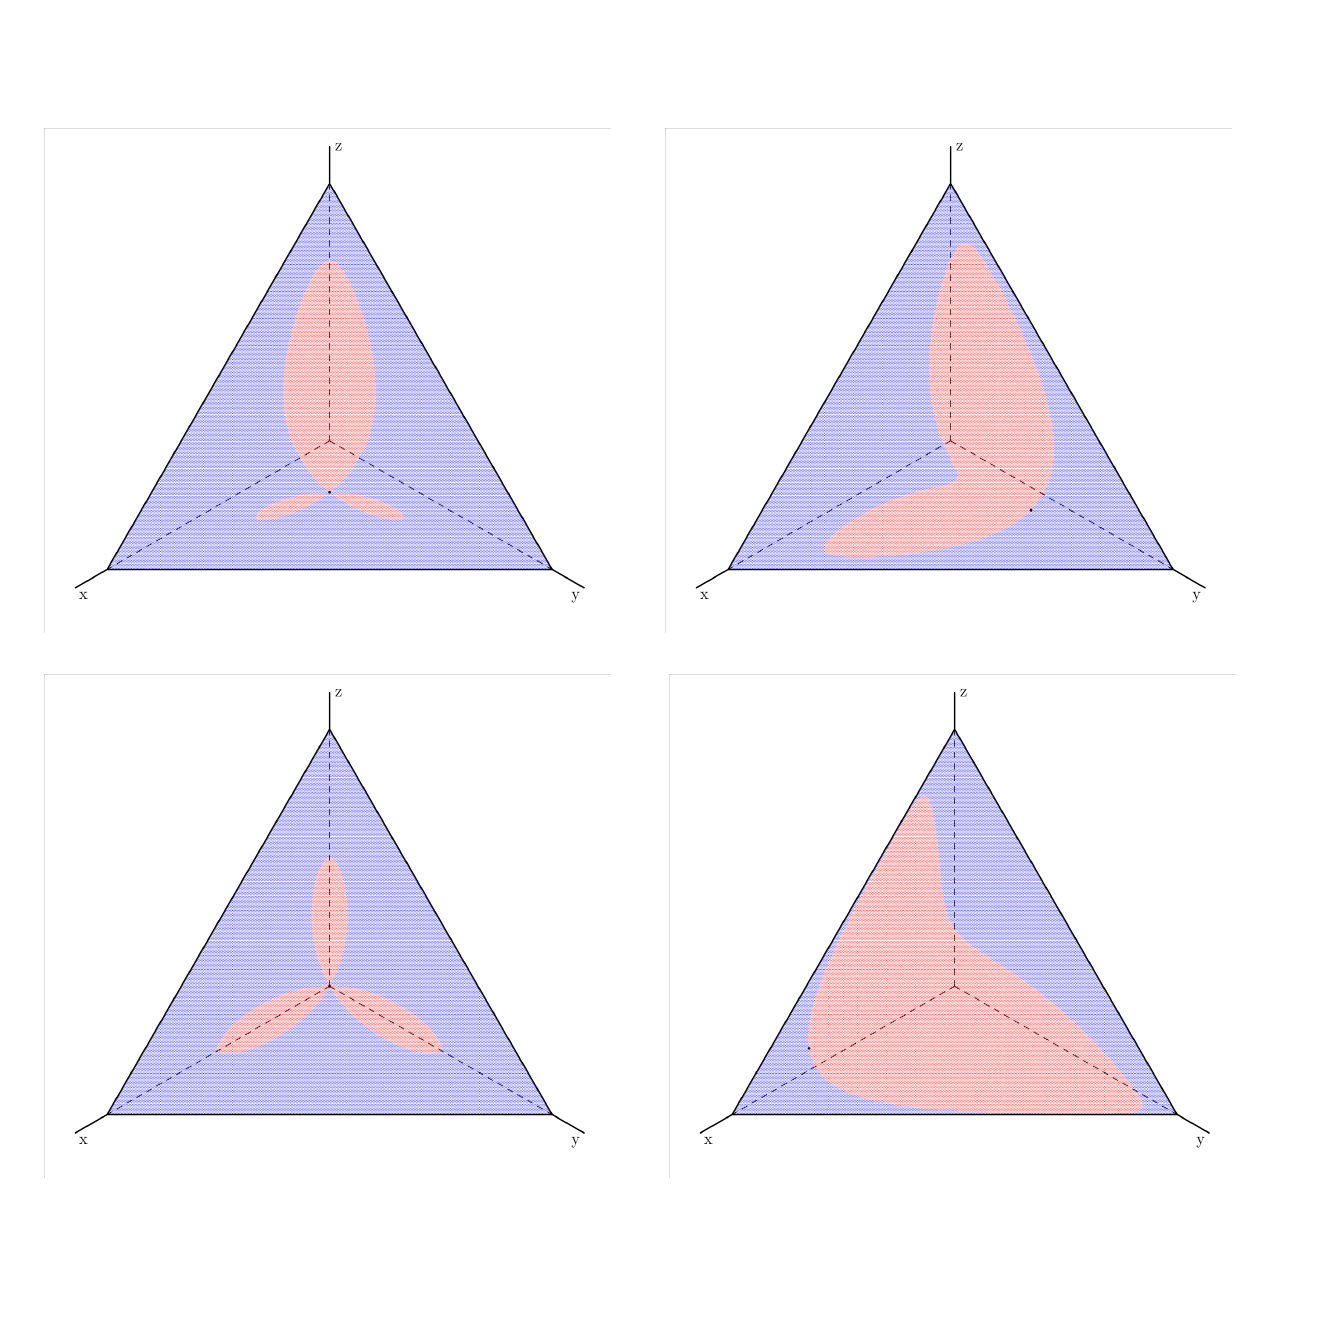
\includegraphics[width=\textwidth]{concat2.png}
      \caption{\footnotesize The partitions induced by equation
        (\ref{eq:sksy}). From top left to bottom right,
        $P=(0.4,0.4,0.2); P=(0.242,0.604,0.154); P=(1/3,1/3,1/3); 
        P=(0.741,0.087,0.172)$.
        Note that for the geometry of reason, the diagrams are
        trivial. The challenge for information theory is to explain
        the non-triviality of these diagrams epistemically without
        begging the question.}
      \label{fig:concat}
    \end{minipage}
  \end{flushright}
\end{figure}

% Lots of good information here: https://en.wikipedia.org/wiki/Information_geometry

% \section{References}
% \label{refs}

% \nocite{*} 
\bibliographystyle{ChicagoReedweb} 
\bibliography{bib-9309}

\end{document}

